\section{\FJ}\label{sec:free-join}

In this section we introduce the \FJ framework.
We start by presenting the Generalized Hash Trie (\GHT) which
 is the data structure used in \FJ (Section~\ref{sec:ght}).
Next we introduce the \FJ plan that specifies 
  how to execute a query with \FJ (Section~\ref{sec:fj-plan}).
Finally, we describe the \FJ algorithm, 
  which takes as input a collection of \GHTs 
  and a \FJ plan,
  and computes the query according to the plan (Section~\ref{sec:free-join-algorithm}).
  
We will show how each of the above components generalizes 
  and unifies the corresponding components in binary join 
  and \GJ: 
  the \GHT generalizes hash tables and hash tries,
  the \FJ plan generalizes binary plans and \GJ plans, and
  the \FJ algorithm generalizes binary join and \GJ.

\begin{figure}
\begin{subfigure}[b]{0.4\linewidth}
\begin{align*}
  Q_{\clubsuit}(x,a,b,c) :- R(x,a),S(x,b),T(x,c)
\end{align*}
\begin{align*}
  R & = \set{(x_0, a_0)} \cup \setof{(x_1, a_i^l), (x_2, a_i^r)}{i \in [1 \ldots n]} \\
  S & = \set{(x_0, b_0)} \cup \setof{(x_2, b_i^l), (x_3, b_i^r)}{i \in [1 \ldots n]} \\
  T & = \set{(x_0, c_0)} \cup \setof{(x_3, c_i^l), (x_1, c_i^r)}{i \in [1 \ldots n]} 
  % R & = \set{(x_0, a_0)} \cup \bigcup_{i \in [1 \ldots n]} \set{(x_1, a_i^l), (x_2, a_i^r)} \\
  % S & = \set{(x_0, b_0)} \cup \bigcup_{i \in [1 \ldots n]} \set{(x_2, b_i^l), (x_3, b_i^r)} \\
  % T & = \set{(x_0, c_0)} \cup \bigcup_{i \in [1 \ldots n]} \set{(x_3, c_i^l), (x_1, c_i^r)} 
\end{align*}
\caption{$Q_\clubsuit$ and inputs.}
\label{fig:clover-query}
\end{subfigure}
\begin{subfigure}[b]{0.5\linewidth}
  \centering
  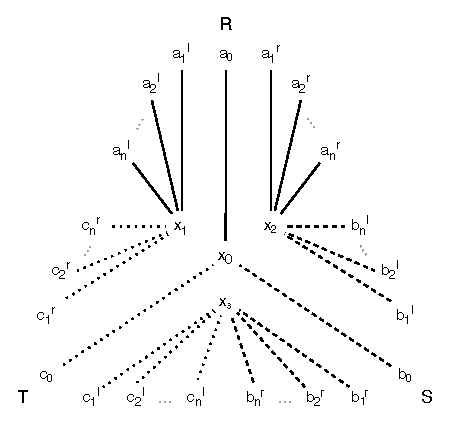
\includegraphics[width=0.8\linewidth]{sand-dollar.pdf}
  \caption{Visualization of the input relations.}
  \label{fig:clover-vis}
\end{subfigure}
\caption{(\ref{fig:clover-query}) the clover query $Q_\clubsuit$, and an input instance.
(\ref{fig:clover-vis}) visualization of the instance in
    Fig.~\ref{fig:clover-query}. The solid (top) edges form the relation
    \texttt{R}, the dashed (right) edges form the relation \texttt{S},
    and the dotted (left) edges form the relation \texttt{T}.  The
    relations join on the attribute in the center.  The only output
    tuple consists of the three edges in the center. }
\end{figure}

Throughout this section we will make use of the {\em clover query}
$Q_\clubsuit$ in Figure~\ref{fig:clover-query}.
Figure~\ref{fig:clover-vis} visualizes the input relations for this query.
Note that $Q_\clubsuit$ is
\emph{acyclic}.

\subsection{The Generalized Hash Trie}\label{sec:ght}

\begin{figure}
\begin{lstlisting}
interface GHT {
  # fields
  relation: String, vars: Vec<String>  
  # constructor
  fn new(name: String, schema: Vec<Vec<String>>) -> Self
  # methods
  fn iter() -> Iterator<Tuple>
  fn get(key: Tuple) -> Option<GHT> }
\end{lstlisting}
\caption{The \GHT interface.}
\label{fig:ght}
\end{figure}

To unify binary join and \GJ, 
  we first need to unify the data structures they work over.
We propose the Generalized Hash Trie 
  which generalizes both the hash table used in binary join 
  and the hash trie used in \GJ.

\begin{definition}[Generalized Hash Trie (\GHT)]
  A \GHT is a tree where each leaf is a vector of tuples, and
  each internal node is a hash map whose keys are tuples, and each key
  maps to a child node.
\end{definition}

We will reuse the terminology defined for tries, including
\emph{level}, \emph{node}, and \emph{leaf}, etc., for \GHTs.  We will
also use the terms \GHT and \emph{trie} interchangeably when the
context is clear.  The {\em schema} of a \GHT is the list
$[\bm y_0,\bm y_1, \ldots, \bm y_\ell]$ where $\bm y_k$ are the
attribute names of the key at level $k$. 

The hash trie used in \GJ is a \GHT where each key is a tuple of size one,
  and the last level stores empty vectors, each of which represents a leaf.
The hash table used in binary join is very similar to a \GHT with only two levels,
  where level 0 stores the keys and level 1 stores
  vectors of tuples.
A small difference is that, in the \GHT, the concatenation of 
  a tuple from level 0 with a tuple from level 1 forms a tuple in the relation, 
  whereas each whole tuple is stored directly in a hash table.
We will show in Section~\ref{sec:colt} how the \COLT data structure
  more faithfully captures the structure of a hash table.
Figure~\ref{fig:ght-examples} shows two examples of \GHTs.

We use \GHTs to represent relations,
  and attach metadata as well as access methods 
  to each \GHT, to be used by the \FJ algorithm.
The \GHT interface is shown in Figure~\ref{fig:ght}.
The \lstinline|relation| field stores the relation name.
A sub-trie inherits its name from its parent.
The \lstinline|vars| field stores parts of the relation's schema:
  if the trie is a vector of tuples, 
  \lstinline|vars| is the schema of each tuple;
  if the trie is a map, 
  \lstinline|vars| is the schema of each key.
The constructor method \lstinline|new| creates a new \GHT from the named relation, 
  where an $n$-th level trie has variables
  matching the $n$-th element of the \lstinline|schema| argument,
  and the values along each path from the root to a leaf of the \GHT 
  form a tuple in the relation.

\begin{example}
  Both \GHTs in Figure~\ref{fig:ght-examples} represent relation $S$ from the
  clover query $Q_\clubsuit$ in Figure~\ref{fig:clover-query}.  The
  \GHT on the left (a hash trie) was created by calling the
  constructor method \lstinline|new| with the schema
  \lstinline|[[x],[b],[]]|, so the top-level trie has the schema
  \lstinline|[x]|, each second-level trie has the schema
  \lstinline|[b]|, and each third-level trie (a leaf) has the empty
  schema \lstinline|[]|.  The \GHT on the right (a hash table) was
  created by calling \lstinline|new| with the schema
  \lstinline|[[x],[b]]|.  It has only two levels, with schema
  \lstinline|[x]| and \lstinline|[b]|, respectively.  Note that each
  $b$ value in the hash trie is hashed and stored as a key, while the
  $b$ values in the hash table are simply stored in vectors.
\end{example}

The methods \lstinline|iter| and \lstinline|get| 
  provide access to values stored in the trie.
If the trie is a map, 
  \lstinline|get(key)| returns the sub-trie mapped to \lstinline|key|,
  if any.
Calling \texttt{get} on a vector returns \lstinline|None|.
If the trie is a vector, 
  \lstinline|iter()|
  returns an iterator over the tuples in the vector;
  calling \texttt{iter} on a map 
  returns an iterator over the keys.

\begin{figure}
  \centering
  \begin{subfigure}[c]{0.3\linewidth}
  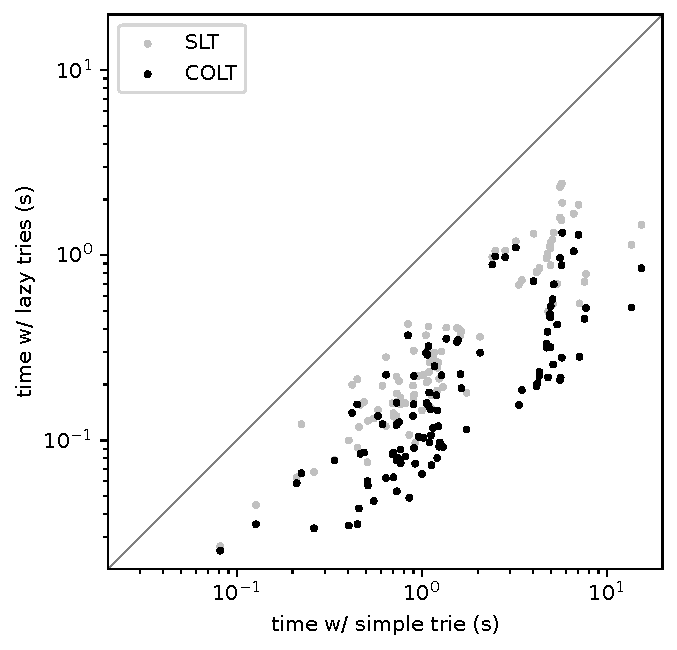
\includegraphics[width=\textwidth]{trie}
  \end{subfigure}\hspace{1.5cm}%
  \begin{subfigure}[c]{0.3\linewidth}
  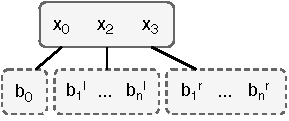
\includegraphics[width=\textwidth]{map}
  \end{subfigure} 
  \caption{
    Two \GHTs. The one on the left is also a hash trie, 
      and the one on the right is similar to a hash table.
    Each box with solid border stores hash keys, 
    and each box with dashed border is a vector of tuples.
    An empty box is an empty vector, representing a leaf.
  }
  \label{fig:ght-examples}
\end{figure}

\begin{example}
  On the second \GHT in Figure~\ref{fig:ght-examples},
    calling \texttt{iter} returns an 
    iterator over the values $[x_0, x_2, x_3]$.
    Calling \texttt{get} with the key $x_2$ 
    returns the sub-trie which is the vector $[b_1^l, \ldots, b_n^l]$.
  Calling \texttt{iter} on this sub-trie
    returns an iterator over $[b_1^l, \ldots, b_n^l]$.
\end{example}


\subsection{The \FJ plan}\label{sec:fj-plan}

% \ds{The section tile doesn't seem right.  What about ``The \FJ plan''}

A \FJ plan specifies how the \FJ algorithm should be executed.
It generalizes and unifies binary join plans and \GJ plans. 
Recall that a left-deep linear plan for binary join
  is a sequence of relations;
  it need not specify the join attributes, 
  since all shared attributes are joined.
In contrast, a \GJ plan is a sequence of variables;
  it need not specify the relations, 
  since all relations on each variable are joined.
A \FJ plan may join on any number of variables and relations at each step,
  and therefore needs to specify both explicitly.

  To help define the \FJ plan, we introduce two new concepts, called
  \emph{subatom} and \emph{partitioning}.  Fix the query $Q$ in
  Eq.~\eqref{eq:cq}:

\begin{definition}
  A \emph{subatom} of an atom $R_i(\bm x_i)$ is an expression
  $R_i(\bm y)$ where $\bm y$ is a subset of the variables $\bm x_i$.
  A \emph{partitioning} of the atom $R_i(\bm x_i)$ is a set of
  subatoms $R_i(\bm y_1), R_i(\bm y_2), \ldots$ such that
  $\bm y_1, \bm y_2, \ldots$ are a partition of $\bm x_i$.
\end{definition}

We now define the \FJ plan using these concepts.

\begin{definition}[\FJ Plan]
  Fix a conjunctive query $Q$.  A \FJ \emph{plan} is a list
  $[\phi_1, \ldots, \phi_m]$, where each $\phi_k$ is a list of
  subatoms of $Q$, called a {\em node}.  The nodes are required to
  {\em partition the query}, in the sense that, for every atom
  $R_i(\bm x_i)$ in the query, the set of all its subatoms occurring
  in all nodes must form a partitioning of $R_i(\bm x_i)$.  We denote
  by $vs(\phi_k)$ the set of variables in all subatoms of $\phi_k$.
  The variables \emph{available to} $\phi_k$ are all variables of the
  preceding nodes:
%
$$avs(\phi_k) = \bigcup_{j < k} vs(\phi_j)$$
%
\end{definition}

%%% Since the partitioning of each atom into subatoms can be inferred 
%%%   from the sequence of nodes, we will omit the partitioning 
%%%   when specifying a \FJ plan.

We will define shortly a {\em valid plan}, but first we show an example.

%%% While a \GJ plan consists of total order of the variables, a \FJ plan
%%% defines only a partial order, if we set
%%% $vs(\Phi_i) < vs(\Phi_2) < \cdots$.


\begin{example}\label{ex:fj-plan}
  The following is an \FJ plan for $Q_\clubsuit$:
\begin{align}
&  [[R(x, a), S(x)], [S(b), T(x)], [T(c)]]\label{eq:bj-plan}
\end{align}
%
To execute the first node we iterate over each tuple $(x, a)$ in $R$
and use $x$ to probe into $S$; for each successful probe we execute
the second node: we iterate over each $b$ in $S[x]$, then use
$x$ to probe into $T$; finally the third node iterates over $c$ in
$T[x]$.  The reader may notice that this corresponds precisely to the
left-deep plan $(R(x,a) \Join S(x,b))\Join T(x,c)$.
%
Another \FJ plan for $Q_\clubsuit$ is: 
%
\begin{align}
  [[R(x), S(x), T(x)], [R(a)], [S(b)], [T(c)]]\label{eq:gj-plan}
\end{align}
%
This plan corresponds to the \GJ plan $[x,a,b,c]$.  Intuitively, here
we start by intersecting $R.x \cap S.x \cap T.x$, then, for each $x$
in the intersection, we retrieve the values of $a$, $b$, and $c$ from
$R$, $S$, and $T$, and output their Cartesian product.
\end{example}

% \begin{figure}
%   \begin{subfigure}[t]{0.4\linewidth}
%     \centering
%     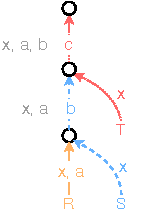
\includegraphics[height=35mm]{fj.pdf}
%     \caption{Plan in Eq.~\eqref{eq:bj-plan} (binary)}
%     \Description[TODO]{TODO}
%     \label{fig:bj-plan}
%   \end{subfigure}
%   \begin{subfigure}[t]{0.5\linewidth}
%     \centering
%     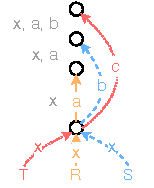
\includegraphics[height=32mm]{gj.pdf}
%     \caption{Plan in Eq.~\eqref{eq:gj-plan} (\GJ)}
%     \label{fig:gj-plan}
%   \end{subfigure}
%   \caption{Visualization of \FJ plans using notations from tensor
%     algebra~\cite{DBLP:journals/pacmpl/KjolstadKCLA17}.  Each circle
%     is a join node.  Arrows pointing to a node indicate the subatoms
%     in that node.  The same color and line style signify the same
%     relation. Grey text shows available variables.}
%   \label{fig:fj-plans}
% \end{figure}

% Readers familiar with tensor algebras may view \FJ as an
% \emph{iteration graph}~\cite{DBLP:journals/pacmpl/KjolstadKCLA17}, as
% shown in Figure~\ref{fig:fj-plans}.  We can ``read off'' the binary
% join plan $[R, S, T]$ from Figure~\ref{fig:bj-plan} by ignoring the
% variables.  Similarly, if we follow the variables in
% Figure~\ref{fig:gj-plan} bottom-up and ignore duplicates, we obtain the \GJ
% plan $[x, a, b, c]$.

Not all \FJ plans are valid, and only valid plans can be executed.  We
execute each \FJ node by iterating over one relation in that node, and
probe into the others.  Therefore, the values used in each probe must
be available, either from the same node or a previous one.

\begin{definition}
  A \FJ plan is \emph{valid} if for every node $\phi_k$ the following
  two properties hold.  (a) No two subatoms share the same relation,
  and (b) there is a subatom containing all variables in
  $vs(\phi_k) - avs(\phi_k)$.  We call such an subatom a \emph{cover}
  for $\phi_k$, and write $cover(\phi_k)$ for the set of covers.
\end{definition}

We will assume only valid plans in the rest of the paper.  To simplify
the presentation, in this section we assume that each node $\Phi_k$,
has {\em one} subatom designated as cover, and will always list it as
the first subatom in $\Phi_k$.  We will revisit this assumption in
Sec.~\ref{sec:optimization}, and allow for multiple covers.

%%% By this definition, every node must contain at least one subatom.  In
%%% addition, since we rename relations in a self-join as described in
%%% Section~\ref{sec:background}, a variable cannot appear in more than
%%% one subatom with the same relation name, and the same variable cannot
%%% appear more than once in the same subatom.

\begin{example}
  Both plans in Example~\ref{ex:fj-plan} are valid.  The covers for
  the 3 nodes for Eq.~\eqref{eq:bj-plan} are $R(x, a)$, $S(b)$, and
  $T(c)$, respectively. For the plan in Eq.~\eqref{eq:gj-plan}, the
  covers for the 4 nodes are $R(x), R(a), S(b), T(c)$; for the first
  node we could have also chosen $S(x)$ or $T(x)$ as cover.
\end{example}
 
% \ds{A few issues in the paragraph above and earlier.  You need to
%   define an atom, since this seems to be nonstandard: I assume you
%   mean that an atom consists of a relation name and a subset of the
%   variables.  The statement ``we do not allow self-joins'' raises
%   eyebrows; I don't think you mean that, please clarify.  The last
%   restriction (no atom contains the same variable twice) is OK, but
%   should be stated and explained in Sec.~\ref{sec:background}.}
% \rw{Will clarify in Backgroud.
%  For self-joins, we do allow them, but we rename the relation names to be different,
%  so that it looks like a join between different relations.
%  I'll also clarify this in Backgroud.  }
% \rw{Add because we rename them.}
% \rw{Use partial atom instead of an atom.}

% \ds{Before the next example add a brief explanation why the plans in
%   Ex.~\ref{ex:fj-plan} are valid.}
\begin{example}
  An example of an \emph{invalid} plan for the clover query has one
  single node containing all relations and variables:
%
  $$[[R(x, a), S(x, b), T(x, c)]]$$
%
  Intuitively, we cannot execute it: if we iterate over, say $R$, then
  we bind two variables $x$ and $a$, but to lookup $S$ we
  need the key $(x,b)$.
\end{example}

% \rw{We partition each atom to subatoms, 
% and define a plan for the query.
% }
% \begin{definition}
%   Given a \FJ plan $[\phi_1, \ldots, \phi_n]$, where 
% $\phi_i = \set{R_1(\overline{x_{i,1}}), \ldots, R_m(\overline{x_{i,m}})}$,
% \FJ computes the query:
% $$Q(*) \cd R_1(\overline{x_{1,1}}, \ldots, \overline{x_{n,1}}), \ldots, R_m(\overline{x_{1,m}}, \ldots, \overline{x_{n,m}}).$$
% That is, for each relation, we concatenate all its variables in the plan in order to form the query. 
% \end{definition}

% \begin{example}
%   Both plans in Eq.~\eqref{eq:bj-plan} and Eq.~\eqref{eq:gj-plan} 
%   compute the clover query $Q(x,a,b,c) \cd R(x,a), S(x,b), T(x,c).$
% \end{example}

% \ds{Add a definition saying ``Given a plan $P$, the query computed by
%   $P$ is $\ldots$'' Then illustrate this defintion with
%   Example~\ref{ex:fj-plan} and the example below.}

% \begin{example}
%   The plan $[\phi=\set{R(), S(), T()}]$ is valid and computes the three-way 
%   Cartesian product of the relations (it does not compute the clover query).
%   The plan is vacuously valid because $vs(\phi) = \emptyset$.
%   Both plans in Eq.~\eqref{eq:bj-plan} and Eq.~\eqref{eq:gj-plan} are also valid.
% \end{example}

% \ds{Equation numbers should be referred to using $\backslash$eqref
%   instead of $\backslash$ref.  I changed them in this file.}

\subsection{Execution of the \FJ Plan}\label{sec:free-join-algorithm}

% \ds{Suggestion: I would call this section ``Execution of the \FJ
%   Plan'' to better connect it to the previous section.}

The execution of a \FJ plan has two phases: the build phase and the
join phase.  The build phase constructs the \GHTs for the relations in
the query, by calling the constructor method \lstinline|new| on each
relation with the appropriate schema.  The join phase works over the
\GHTs to compute the join of the relations.

% fn ght_schema(relation, plan):
%   schema = []
%   for node in plan:
%     for atom in node:
%       if atom.relation == relation:
%         schema.append(atom.variables)
%   return schema 

\begin{figure}
  \begin{lstlisting}[
    commentstyle=\color{gray},
    escapeinside={(*}{*)},
    ]
fn join(all_tries, plan, tuple):
  if plan == []:
    output(tuple) (* \label{lst:output} *)
  else:
    tries = [ t $\in$ all_tries | t.relation $\in$ plan[0] ] (* \label{lst:select} *)
    # iterate over the cover
    @outer for t in tries[0].iter(): (* \label{lst:outer} *)
      subtries = [ iter_r.get(t) ] (* \label{lst:inner} *)
      tup = tuple + t
      # probe into other tries
      for trie in tries[1..]:     
        key = tup[trie.vars] (* \label{lst:key} *)
        subtrie = trie.get(key)
        if subtrie == None: continue @outer
        subtries.push(subtrie) (* \label{lst:inner-end} *)
      new_tries = all_tries[tries $\mapsto$ subtries] (* \label{lst:tuple} *)
      join(new_tries, plan[1:], tup) (* \label{lst:join} *)
\end{lstlisting}
  \caption{The \FJ algorithm.}
  \label{fig:fj-algo}
\end{figure}

\subsubsection*{Build Phase}
The build phase constructs a \GHT for each relation (atom)
$R_i(\bm x_i)$, as follows.  If the plan partitions the atom into the
subatoms $R_i(\bm y_0), R_i(\bm y_1), \ldots, R_i(\bm y_{\ell-1})$,
then the schema of its \GHT is the list
$[\bm y_0, \bm y_1, \ldots, \bm y_{\ell-1}, []]$.  Recall that the
last level of a \GHT is a vector instead of a hash map. As an
optimization, if the last subatom $R_i(\bm y_{\ell-1})$ is the cover
of its node, then we drop the last $[]$ from the schema, in other
words, we construct a vector for the $\bm y_{\ell-1}$.  After
computing the schema for each relation, we call the constructor method
\lstinline|new| on each relation and its computed schema to build the
\GHTs.

\begin{example}
  Consider the plan in Eq.~\eqref{eq:bj-plan} for the clover query
  $Q_\clubsuit$.  The \GHT schemas for $R$, $S$, and $T$ are
  $[[x, a]]$, $[[x], [b]]$, and $[[x], [c]]$ respectively.  Thus, $R$
  is a flat vector of tuples, and each of $S$ and $T$ is a hash map of
  vectors of values.  Consider now the triangle query $Q_{\triangle}$
  and the plan $[[R(x,y),S(y),T(x)],[S(z),T(z)]]$.  The \GHT
  schemas for $R, S, T$ are $[[x,y]]$, $[[y],[z]]$, and $[[x],[z],[]]$:
  in other words $R$ is stored as a vector, $S$ is a hash-map of
  vectors, and $T$ is a hash-map of hash-maps of vectors.
\end{example}

\subsubsection*{Join Phase}
The pseudo-code for the \FJ algorithm is shown in Figure~\ref{fig:fj-algo}.
The \lstinline|join| method takes as input the \GHTs, the \FJ plan, 
  and the current tuple initialized to be empty.
If the plan is empty, we output the tuple (line~\ref{lst:output}).
Otherwise, we work on the first node in the plan
  and intersect relevant tries (line~\ref{lst:select}).
We iterate over tuples in the covering relation, 
  which is the first trie in the node (line~\ref{lst:outer}).
%
% First we pick the trie to iterate over (line~\ref{lst:iter}).
% If any trie is a vector, we iterate over it.
% % \dan{I think it's clearer if you always iterate over the first
% %   subatom, which is the cover of the node.  We just need to make sure
% %   that this subatom is a vector, when that's possible.}
% % For now, we assume for each join node, at most one trie is a vector.
% % %
% % \yell{At this point there is nothing left to assume.  The \GHT is well
% %   defined, and only its last level is a vector, and the \GHT schema
% %   for a plan is well defined.  Everything is well defined.}
% % %
% We will relax this assumption in Section~\ref{sec:colt}.
% If all tries are hash maps, we iterate over the one with the fewest keys.
% After picking the trie to iterate over, 
%   we sort the other tries by some estimated cost to probe into them (line~\ref{lst:probe}).
% For example, we can probe into the smaller trie first, 
%   since it is likely to be selective, and may fit into the cache.
%
% In the outer for loop (line~\ref{lst:outer})
%   we iterate over each tuple \lstinline|t| in the trie we have picked.
Then, we use values from \lstinline|t| 
  and the \lstinline|tuple| argument
  as keys to probe into the other tries 
  (line~\ref{lst:inner}-\ref{lst:inner-end}).
To construct a key for a certain trie, 
  we find the values mapped from the trie's schema variables
  in \lstinline|t| and \lstinline|tuple| (line~\ref{lst:key}).
If any probe fails, we continue to the next tuple in the outer loop.
If all probes succeed, we replace the original tries with the 
  subtries returned by the probes,
  and recursively call \lstinline|join| 
  on the new tries and the rest of the plan (line~\ref{lst:tuple}-\ref{lst:join}).

The recursive definition may obscure the essence of the \FJ algorithm,
  so we provide some examples where we unroll the recursion.
We introduce some convenient syntax to simplify the presentation.
We write \lstinline|for (x,y,...) in T:| 
  to introduce a for-loop iterating over \lstinline|T|, 
  binding the values of each tuple in \lstinline|T.iter()| 
  to the variables \lstinline|x,y,...|.
We write \lstinline|r = R[t]?| to bind the result of 
  \lstinline|R.get(t)| to \lstinline|r|;
  if the lookup fails, we continue to the next iteration of the 
  enclosing loop.
In other words, \texttt{r = R[t]?} is equivalent to:
%
\begin{lstlisting}
r = R.get(t); if r.is_none(): continue
\end{lstlisting}

\begin{figure*}
  \begin{subfigure}[b]{0.3\linewidth}
\begin{lstlisting}[escapeinside={(*}{*)}]
R = GHT("R",[["x","a"]])
S = GHT("S",[["x"],["b"]])
T = GHT("T",[["x"],["c"]])
for (x, a) in R:
  s = S[x]?
  for b in s:
   (* \underline{t = T[x]?} *)
    for c in t:
      output(x, a, b, c)
\end{lstlisting}
    \caption{Binary \FJ.}
    \label{fig:bj-loop}
  \end{subfigure}
\hspace{1.5em}
  \begin{subfigure}[b]{0.3\linewidth}
    \centering
\begin{lstlisting}[
    escapeinside={(*}{*)}
]
# same as the left
# ...
# ...
for (x, a) in R:
  s = S[x]?
 (* \underline{t = T[x]?} *)
  for b in s:
    for c in t:
      output(x, a, b, c)
\end{lstlisting}
    \caption{Factorized \FJ.}
    \label{fig:factorized-loop}
  \end{subfigure}
  \hspace{.5em}
  \begin{subfigure}[b]{0.3\linewidth}
    \centering
\begin{lstlisting}
R = GHT("R",[["x"],["a"]])
# same as the left
# ...
for x in R:
  r=R[x]?; s=S[x]?; t=T[x]?
  for a in r:
    for b in s:
      for c in t:
        output(x, a, b, c)
\end{lstlisting}
    \caption{Generic \FJ.}
    \label{fig:gj-loop}
  \end{subfigure}
  \Description[TODO]{TODO}
  \caption{Execution of \FJ for the clover query.}
\end{figure*}

\begin{example}\label{ex:binary-free-join}
  Consider the plan in Eq.~\eqref{eq:bj-plan} for the clover query $Q_\clubsuit$.
  Figure~\ref{fig:bj-loop} shows its execution; ignore the underlined
  instruction for now.
%%%   Here we have omitted all ``setup'' code, 
%%%     showing only the nested loops performing iteration and lookup.
  In the build phase, 
    we construct a flat vector for $R$ and a hash table for each of $S$ and $T$.
  In the join phase, for the  node $[R(x, a), S(x)]$  we 
   iterate over $R$ and probe into $S$, while for the second node $[S(b), T(x)]$,
    we iterate over the second level of $S$ and probe into $T$.
  Finally, the third loop iterates over the second level of $T$ and outputs the result.
\end{example}

\begin{example}\label{ex:generic-free-join}
  Consider now the plan in Eq.~\eqref{eq:gj-plan} for  $Q_\clubsuit$.
  Its execution is shown in Figure~\ref{fig:gj-loop}.
  We construct  hash tables for $R$, $S$, and $T$, keyed on $x$.
  The first loop level intersects the three relations on $x$, 
    and subsequent loop levels take the Cartesian product of the relations on $a$, $b$, and $c$.
\end{example}

Note that Fig.~\ref{fig:bj-loop}
  follows the execution of binary hash join with the plan $[R, S, T]$,
  whereas Fig.~\ref{fig:gj-loop} follows the execution of \GJ
   with the plan $[x, a, b, c]$.  We will describe
   Fig.~\ref{fig:factorized-loop} later.

\subsection{Discussion}

\FJ plans generalize both traditional binary plans and \GJ.  
% We will describe in the next section a simple optimization that allows us to
% cover the full spectrum in Fig.~\ref{fig:design-space}.  
One
limitation so far is our assumption that the cover is chosen during
the {\em build phase}.  This was convenient for us to illustrate how
to avoid constructing some hash maps, by storing the last level of a
\GHT as vector, when it corresponds to a cover.  In contrast, \GJ
computes the intersection $R_1.x\cap R_2.x\cap \cdots$ by iterating
over the smallest set, hence it chooses the ``cover'' at run time.  We
will address this in the next section by describing \COLT, a data
structure that constructs the \GHT lazily, at run time, allowing us to
choose the cover during the {\em join phase}.
